\def\layersep{2.5cm}
\def\nodeinlayersep{1.2cm}
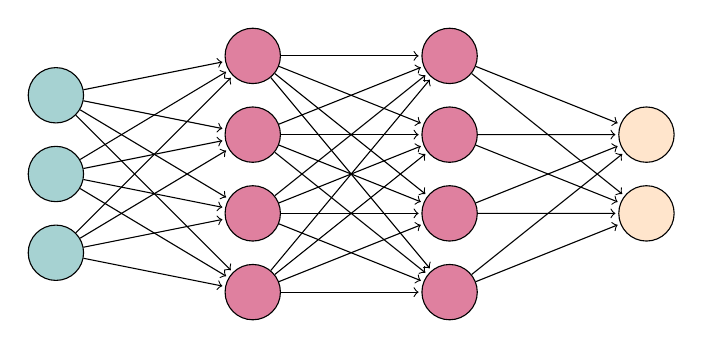
\begin{tikzpicture}[shorten >=1pt,->, node distance=\layersep]
    \tikzstyle{every pin edge}=[<-,shorten <=1pt]
    \tikzstyle{neuron}=[draw, circle, fill=black!25,minimum size=20pt,inner sep=0pt]
    \tikzstyle{input neuron}=[neuron, fill=teal!35];
    \tikzstyle{output neuron}=[neuron, fill=orange!20];
    \tikzstyle{hidden neuron}=[neuron, fill=purple!50, minimum size=20pt];
    \tikzstyle{hidden neuron2}=[neuron, fill=purple!50, minimum size=20pt];

    \foreach \name / \y in {0,...,2}
        \node[input neuron] (I-\name) at (0,-\y) {};

    \foreach \name / \y in {0,...,3}
        \path[yshift=0.5cm]
            node[hidden neuron] (H1-\name) at (\layersep,-\y cm) {};

    \foreach \name / \y in {0,...,3}
        \path[yshift=0.5cm]
            node[hidden neuron2] (H2-\name) at (2*\layersep,-\y cm) {};    

    \foreach \name / \y in {0,...,1}
        % \node[output neuron,pin={[pun edge={->}]right:Output \#\y}, right of=H2-2] (O-\name) at (3*\layersep, -\y cm) {};
        \path[yshift=-0.5cm]
            node[output neuron] (O-\name) at (3*\layersep, -\y cm) {};


    \foreach \source in {0,...,2}
        \foreach \dest in {0,...,3}
            \path (I-\source) edge (H1-\dest);

    \foreach \source in {0,...,3}
        \foreach \dest in {0,...,3}
            \path (H1-\source) edge (H2-\dest);

    \foreach \source in {0,...,3}
        \foreach \dest in {0,...,1}
            \path (H2-\source) edge (O-\dest);
\end{tikzpicture}